\documentclass[../m2r-report.tex]{subfile}

The idea of finding regular behaviour from apparent chaos is immediately
applicable to graphs.
The statement in the introduction - ``Given 6 people, either 3 mutually know each
other, or 3 do not" - can be rephrased in a graph theoretic sense.
We identify a person with a vertex of the graph, and a relation between them as
an edge.
A relation between two people can have two states: either the two know each other,
or they have never met.
We can illustrate this relation status by `colouring' the edge, with a red edge
showing that the two know each other, and a blue edge showing that they haven't.
Hence, the situation described by the statement is shown by the following graph:

\begin{figure}[h]
\begin{center}
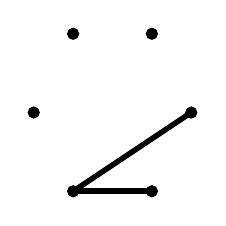
\begin{tikzpicture}
    \draw[line width=2pt] (0,0) -- (1,0);
    \draw[line width=2pt] (0,0) -- (1.5,1);

    \filldraw (0,0) circle (2pt);
    \filldraw (1,0) circle (2pt);
    \filldraw (-0.5,1) circle (2pt);
    \filldraw (1.5,1) circle (2pt);
    \filldraw (0,2) circle (2pt);
    \filldraw (1,2) circle (2pt);

\end{tikzpicture}
\caption{An arbitrary 2-colouring of $K_6$}
\end{center}
\end{figure}

This graph describes a situation in which we have two disjoint sets of 3 people
which mutually do not know each other, illustrated by the two blue triangle which
lie within the graph.


